\chapter{Alignments with Pair HMMs}

In this chapter we will describe scoring schemes for pair alignment using PHMMs.
We can divide states of PHMM into three types.  Ones that generates symbol in
both sequences, states that generates symbol in only one sequence and silent
states. If PHMM generates  symbols in both sequences we consider those symbols
to be homologous. We will consider symbols that were not generated by such state
as indels.

If we have sequences $X$ and $Y$, probability $\prob{X,Y\mid H}$ is the
probability, that $X$ and $Y$ are aligned according model $H$. Since from state
path $\pi$ we can reconstruct unique alignment, we will denote $\pi$ also as an
alignment. $\prob{\pi\mid X,Y,H}$ is the probability, that $\pi$ is alignment of
$X$ and $Y$ under the condition, that $X$ and $Y$ were generated by model
$H$. We can use $\prob{\pi\mid X,Y,H}$ as a score of an alignment $\pi$. Later
in this chapter we show how to derive different scoring functions.


\section{Simple Pair HMM  Model}\label{SECTION:SIMPLEPHMM}

We show classical PHMM for sequence alignment. It is equivalent to scoring
scheme of Needleman-Wunch algorithm with affine gap model. It consists of three
states: one that generates aligned pairs, and two states for generating
indels (one for each sequence). Model is shown in figure \ref{PHMM:FIG:SIMPLEPHMM}. 

\begin{figure}[Simple pair HMM model for alignment.]
\begin{center}
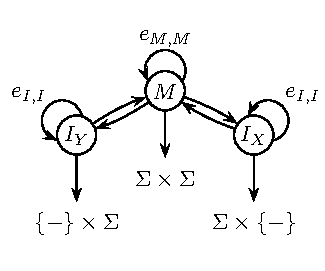
\includegraphics{../figures/pairHMM.pdf}
\end{center}
\caption{Pair hidden Markov model for pair alignment. It has two transitions
parameters $e_{M,M}$ and $e_{I,I}$, since we set $e_{I,M} = 1 - e_{I,I}$ and
$e_{M,I}=\frac12-\frac12e_{M,M}$. Match state $M$ generates aligned pair of symbols
and states $I_X$ and $I_Y$ generates symbols only in $X$ or $Y$ respectively.
Initial distribution is even.
}\label{PHMM:FIG:SIMPLEPHMM}
\end{figure}

As mentioned before, score of the alignment is the probability of state path
that correspond to such alignment. Therefore we can find the alignment with 
highest score by two dimensional version of Viterbi algorithm. 

\section{More Complex models}

In this section we will review several PHMMs and GPHMMs that were used to
sequence alignment or other purpose, for example gene finding. We will review
the application domain of the model, its topology, decoding function, parameter
estimation and optimisation heuristics. But at first, we have to introduce small
biological background.

TODO: Tu bude mega obrazok (asi na jednu stranu), kde budu nakreslene rozne
topologie.

\subsection{Genes}

Gene, codon, exon, intron, triplets,..., evolution rate, splice site

\subsection{DoubleScan}
Meyer {\it et al. (2002)} developed gene finder, that used evidence from the
sequences of two organism to find genes. Their GPHMM has 54 states. Generally,
they have three types of states: {\it match} states, which generated same number
of symbols in both sequences;   {\it emit} states, which generate sequences only
in one sequence and silent states. DoubleScan's HMM contains structures for
exons, introns and intron-like structures that are outside genes. Every such
structure has three version: one matching version, which emit aligned residues
and one structure per sequence to emit indels.  Overview of DoubleScan's HMM
structure is in figure \ref{}. 
\nocite{Meyer2002}

Emission probabilities if the {\it match exon} state were estimated from
relating frequencies in the training set with Dirichlet priors.
Emission probabilities of other states were generated  by marginalizing
emissions of the match exon state. Transition probabilities from begin state
were even, transition probabilities for splice sites were estimated from splice
site predictor and other transitions were observed from train data and tuned by
hand.

DoubleScan uses Viterbi algorithm as decoding method.  To reduce running time of
Viterbi algorithm they use stepping stone algorithm: at first they run BLASTN to
find local alignments. Then DoubleScan choose consistent subset of matching by
greedy method. They restrict Viterbi algorithm to such subset allowing with
tolerance of 15 bases.

\subsection{SLAM}

SLAM is comparative-based gene finder \cite{SLAM2003} based on generalized pair
hidden Markov model \cite{Alexanderson2004} with some states being also a
high-order states (with dependence on previous emissions).  It predicts gene
structures for pair of related eukaryotic organisms. SLAM's decoding method is
Viterbi algorithm. 

Unlike DoubleScan, SLAM defines true GPHMM because states at first generates
duration times according geometric distribution and after that they emit
sequences. SLAM's topology can by found in picture \ref{}. \todo{Ako pozeram,
tak pozeram, ta ich toplogia mi teda neni jasna}

Emission of pairs of codons were assigned from codon-based PAM matrix. Exon
states were fifth order states.

To reduce running time of the algorithm, they restrict computation of alignment
in following way: At first they  align input sequences using AVID alignment
tool\cite{} to get anchor alignment. They restrict Viterbi algorithm in such
way, that it could align  in a way, that every base from  bases were extended to
intervals of size $3$ bases of bases surrounding each matching base.



\subsection{Twine}

Twain is another approach to use GPHMM (and evidence from two related genomes) to gene
finding \cite{Majoros2005}. 



\subsection{GeneWise}

GeneWise is protein (or profile HMM) to DNA aligner \cite{Birney2004}. It aligns
proteins to homologous exons in DNA. Instead of PHMM defined as in chapter
\ref{}, it used probabilistic transducers (which are similar to PHMM). Main
difference in their model was that emissions were defined for transitions and
not for states.  It's model was created by combining of the gene prediction
model (model $S$) and protein homology model (model $T$). Both models were
represented as PHMM or \correction{transducers}{Napis co to je v kapitole o
HMM}. While model $S$ translates DNA into protein sequence, $T$ was simple PHMM
from section \ref{SECTION:SIMPLEPHMM} defined over protein alphabet
(technically, $T$ translates one protein to another homologous protein).
Combined model was created by composition of models $T$ and $S$, from which were
removed unnecessary states. To decrease state space even more, they remove more
states, for example poly-pyrimidine states. More details are in
\cite{Birney2004}.

Parameters for match and insert transitions were derived from amino acid
distribution from the model $T$, from the codon bias in the organism and there
was allowed one substitution error while translating codons to amino acids (due
sequencing errors).
 
\subsection{Pairagon}

Pairagon alignes \abbreviation{coding DNA}{cDNA} to  genome \cite{Pairagon2009}.
To do this task, Pairagon's HMM models consists from simple pair HMM submodel,
which aligns cDNA to DNA and 5 state submodel for intron structures (donor site,
intron, branch, branch acceptor and acceptor state). This model includes 8 base
\abbreviation{weighted matrix model}{WMM} at donor site and 6 base WMM at
acceptor size. Whole topology is in figure \ref{}.

Model was trained using iterative maximum likelihood approach. At first they
trained almost all parameters on BLAT alignments from the
\abbreviation{Mammalian Gene Collection}{MGC}. In this phase, probabilities of
canonical intron, the branch point and the sequence models were set by hand.
After that they used estimated parameters to align more MGC sequences, from
which were the rest of the parameters estimated.

Decoding was done by Viterbi algorithm. Runtime of the algorithm was improved by
stepping stone algorithm \cite{} and memory requirements were improved using
Treeterbi algorithm. 


\subsection{FEAST}
FEAST is pairwise local alignment tool \cite{FEAST2011}. Simple PHMM from figure
\ref{PHMM:FIG:SIMPLEPHMM} is optimized for one fixed rate of evolution. However,
in DNA conservation rate is different on different sites.  FEAST contain $k$
such submodels, each trained for different rate of evolution, each of them
connected with single silent state. Since FEAST is local alignment tool, it
one additional submodel for generating unaligned sequences (once PHMM enters
such model, it won't leave). Model topology is described in picture
\ref{}.

To construct alignment (either local or global) FEAST uses the Viterbi
algorithm. Like many local aligners, FEAST at first use six different space
seeds to get hits and extended those hits using x-drop heuristic \cite{}.
However, they use ungapped version of Forward algorithm during extension
(Viterbi algorithm is usually used during extension phase).

Estimation of parameters was done by expectation maximization approach (with
Baum-Welch or Viterbi training). They forced gap parameters to be same in all
submodels.


Dalsie modely: TWINSCAN, MCALIGN2, WABA, Catwright (zeta function)

\section{More Complex Gap Models}
Gapmodel defined by PHMM is in fact affine gapmodel.
Gap length have geometric distribution: the probability that gap have length $d$
is $e_{M,I}e_{I,I}^{d-1}(1-e_{I,I})$ (if we sum out all emissions). However,
using
%co chcem povedat: niekedy je lepsie pouzit iny gapmodel -- jeden pre kratke
%gapy, jeden pre slhe gapy. Preto sa niekedy 

